\documentclass[12pt, a4paper, oneside]{ctexart}
\usepackage{amsmath, amsthm, amssymb, bm, color, framed, graphicx, hyperref, mathrsfs}

\title{\textbf{3月30日作业}}
\author{韩岳成 524531910029}
\date{\today}
\linespread{1.5}
\definecolor{shadecolor}{RGB}{241, 241, 255}
\newcounter{problemname}
\newenvironment{problem}{\begin{shaded}\stepcounter{problemname}\par\noindent\textbf{题目\arabic{problemname}. }}{\end{shaded}\par}
\newenvironment{solution}{\par\noindent\textbf{解答. }}{\par}
\newenvironment{note}{\par\noindent\textbf{题目\arabic{problemname}的注记. }}{\par}
\everymath{\displaystyle}

\begin{document}

\maketitle

\begin{problem}
    两人在图 $G$ 上做游戏：交替选择相异的顶点 $v_0, v_1, v_2, \dots$，使得对每个 $i > 0$，$v_i$ 与 $v_{i-1}$ 相邻，选择最后一个顶点者获胜。证明：第一选点人有一个得胜策略当且仅当图 $G$ 没有完美匹配。
\end{problem}

\begin{solution}
   游戏过程实质上是在图 $G$ 中构造一条路径 $P = (v_0, v_1, v_2, \dots)$。

\textbf{必要性:}
反证假设图 $G$ 存在一个完美匹配 $M$。

第一选点人选择任意顶点 $v_0$。由于 $M$ 是完美匹配，根据定义，存在唯一的边 $(v_0, v_1) \in M$。第二选点人只需选择 $v_1$。

此后，对于第一选点人选择的任意顶点 $v_{2k}$，由于 $M$ 中包含 $(v_{2k}, v_{2k+1})$，第二选点人总能选择 $v_{2k+1}$。

因为 $M$ 覆盖了图中的所有顶点，只要第一选点人能够移动，第二选点人必然能通过匹配边做出对应移动。因此，游戏最终必将由第二选点人落下最后一子，即第二选点人有必胜策略，第一选点人没有必胜策略，与题设矛盾。

因此，若先手有必胜策略，则图 $G$ 必定没有完美匹配。

\textbf{充分性:}
设 $M$ 为图 $G$ 的一个最大匹配。若 $G$ 没有完美匹配，由 Berge 定理可知，必然存在至少一个 $M$-非饱和顶点。

\textbf{第一选点人的策略}：
\begin{enumerate}
    \item 第一步，选点人选择一个 $M$-非饱和顶点 $v_0$。
    \item 此后，每当第二选点人选择了顶点 $v_{2k+1}$ 后，第一选点人总是选择顶点 $v_{2k+2}$，使得 $(v_{2k+1}, v_{2k+2}) \in M$。
\end{enumerate}

我们通过归纳法证明：在每一轮第一选点人行动前，$v_{2k}$ 均是 $M$-饱和的，且第一选点人总能找到符合条件的 $v_{2k+2}$。

第一选点人选择非饱和点 $v_0$。第二人被迫选择一个与 $v_0$ 相邻的 $v_1$。此时边 $(v_0, v_1)$ 必然不属于 $M$（因为 $v_0$ 不被 $M$ 覆盖）。由于 $M$ 是最大匹配，$v_1$ 必然是 $M$-饱和的，否则 $(v_0, v_1)$ 是一个没有包含在$M$中的匹配边，与最大匹配矛盾。因此，存在唯一的 $v_2$ 使得 $(v_1, v_2) \in M$。第一人选择 $v_2$。
    
假设第一人已完成 $v_{2k}$ 的选择，$v_{2k}$ 为 $M$-饱和点。第二人选择与 $v_{2k}$ 相邻的 $v_{2k+1}$。由于 $(v_{2k-1}, v_{2k}) \in M$，为了保证路径相异，$v_{2k+1}$ 只能通过一条非匹配边与 $v_{2k}$ 相连。同理，若 $v_{2k+1}$ 是 $M$-非饱和的，则 $(v_0, v_1, \dots, v_{2k+1})$ 构成一条增广路径，这与 $M$ 是最大匹配矛盾。因此，$v_{2k+1}$ 必然是 $M$-饱和的。故存在唯一的 $v_{2k+2}$ 使得 $(v_{2k+1}, v_{2k+2}) \in M$。第一人选择该 $v_{2k+2}$ 即可。

由于图是有限的且 $M$ 中每条边最多被访问一次，游戏最终必然终止。由于第一选点人始终能够通过 $M$ 中的匹配边进行回应，最后无法移动的必为第二选点人。因此，第一选点人有必胜策略。
\end{solution}

\begin{problem}
下图所示的是 14 个大小相同的正方形组成的图形。试证明：不论如何用剪刀沿着图形中所画的直线对它进行裁剪，总剪不出 7 个由相邻的两个小正方形组成的矩形。

\begin{center}
    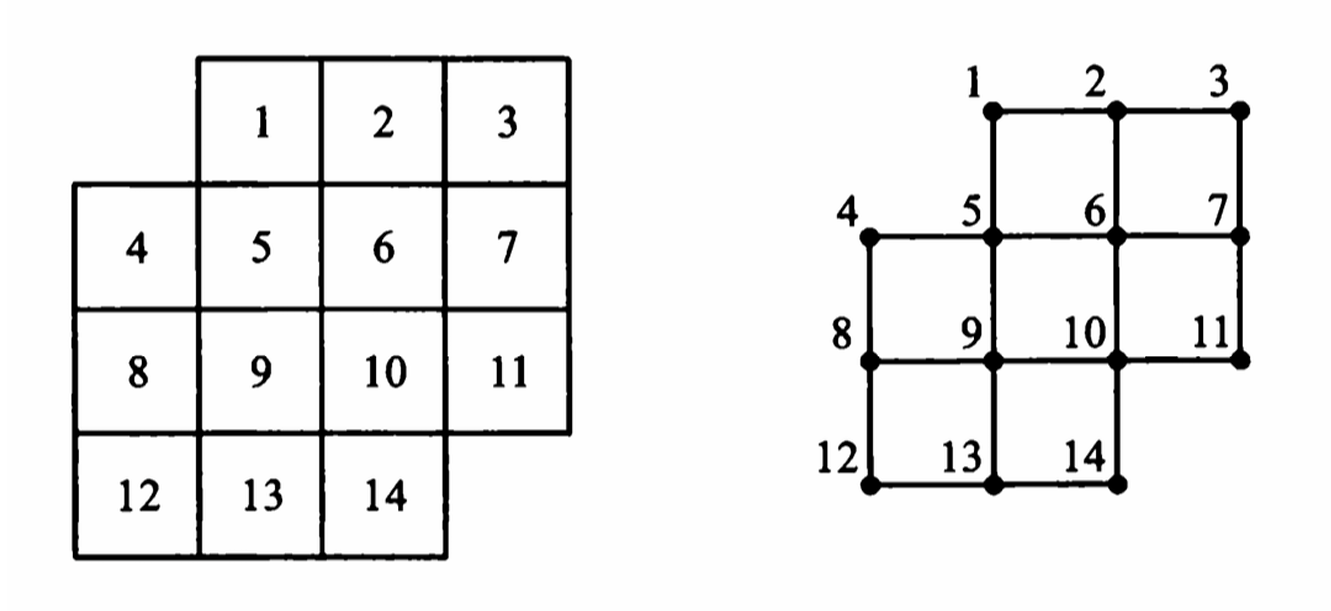
\includegraphics[width=0.62\textwidth]{image.png}
\end{center}
\end{problem} 

\begin{solution}
该问题等价于在右图中找出一个含有7条边的匹配能够覆盖全部14个顶点。我们将证明这个完美匹配不存在。

观察可得右图为二部图，设左侧顶点集合为 $A = \{1,3,4,6,9,11,12,14\}$，右侧顶点集合为 $B = \{2,5,7,8,10,13\}$。每条边连接一个 $A$ 中的顶点和一个 $B$ 中的顶点。

根据霍尔定理，对于二部图 $G = \left \langle A \cup B, E \right \rangle $，$G$有饱和顶点子集$A$中所有顶点的匹配当且仅当对于任意顶点子集$S \subseteq A$，其邻域$N(S)$满足$|N(S)| \ge |S|$。

我们取$S = A$，则$N(S) = B$，满足$|N(S)| = 6 < 8 = |S|$。因此，存在一个匹配无法覆盖 $A$ 中的所有顶点。

则不存在一个匹配能够覆盖 $A$ 中的所有 8 个顶点，因此也不可能存在一个匹配能够覆盖全部 14 个顶点。
\end{solution}


\end{document}